
\begin{center}
\LARGE\textbf{PI Summary: Jonathan Asaadi}
\end{center}

%%%%%%%%%%%%%%%%%%%%%%%%%%%%%%%%%%%%%%%%%%%%%%%%5
\section*{\textbf{Accomplishments}}
%%%%%%%%%%%%%%%%%%%%%%%%%%%%%%%%%%%%%%%%%%%%%%%%%

\noindent\textbf{LArIAT Experiment}

\begin{itemize}[noitemsep,nolistsep]
\item{\textbf{LArIAT Co-Spokesperson}}: Beginning September 2016

\item{\textbf{LArIAT Analysis Coordinator}}: Lead the first measurement of the inclusive $\pi^{-}$-Argon cross-section shown in Figure \ref{fig:LArIATCrossSection} (paper in preparation).

\begin{figure}[htb]
\centering
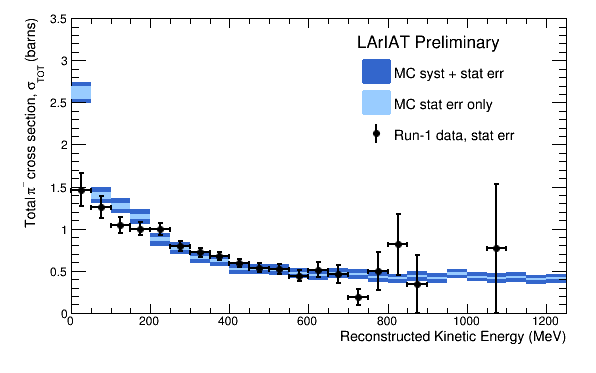
\includegraphics[width=0.55\textwidth]{images/LArIATCrossSection.png}
\caption[]{First inclusive $\pi^{-}$-Argon cross-section.}
\label{fig:LArIATCrossSection}
\end{figure}


\end{itemize}

\noindent\textbf{MicroBooNE Experiment}
\begin{itemize}[noitemsep,nolistsep]
\item{\textbf{TPC Commissioning Coordinator}}: Developed and executed the commissioning plan for the MicroBooNE TPC

\item{\textbf{Lead TPC Expert}}: Develop the expert documentation for the TPC and coordinate the expert shifts

\item{\textbf{Astro-Particle and Exotics Working Group Convener}}: Lead one of the MicroBooNE working groups and contribute to a preliminary proton decay background analysis \cite{}.

\end{itemize}

\noindent\textbf{ArgoNeuT Experiment}
\begin{itemize}[noitemsep,nolistsep]
\item{\textbf{Lead Analyzer on the ``Measurement of $\nu_{\mu}$ and $\bar{\nu}_{\mu}$ Neutral Current $\pi^{0} \rightarrow \gamma\gamma$ Production in the ArgoNeuT Detector''}} : First measurement of NC-$\pi^{0}$ production on argon

\item{\textbf{Contributer to ``First Observation of Low Energy Electron Neutrinos in a Liquid Argon Time Projection Chamber''}}: Paper in preparation

\end{itemize}





\noindent\textbf{University of Texas Arlington}

\begin{itemize}[noitemsep,nolistsep]
\item{\textbf{Establishment of Cryogenic Laboratory}}: Building a facility capable of purifying and recirculating liquid argon for use in detector R$\&$D and testing.
\end{itemize}

%%%%%%%%%%%%%%%%%%%%%%%%%%%%%%%%%%%%%%%%%%%%%%%%%
\section*{\textbf{Milestones}}
%%%%%%%%%%%%%%%%%%%%%%%%%%%%%%%%%%%%%%%%%%%%%%%%%
\noindent\textbf{protoDUNE Experiment}
\begin{itemize}[noitemsep,nolistsep]
\item{\textbf{APA QA/QC Documentation and Testing}}: Early 2017
\item{\textbf{Detector Installation, Commissioning, and Operations}}: Late 2017-2018
\item{\textbf{Data Taking and Analysis}}: Mid 2018 - 2019
\end{itemize}

\noindent\textbf{SBND Experiment}
\begin{itemize}[noitemsep,nolistsep]
\item{\textbf{Cold Electronics Test Stand}}: Delivery to FNAL Summer 2017
\item{\textbf{Detector Construction}}: Mid 2017 - Mid 2018
\item{\textbf{Commissioning and Data Taking}}: Starting Mid 2018 
\item{\textbf{Cross-Section Analysis}}: Preliminary studies beginning late 2019

\end{itemize}

\noindent\textbf{MicroBooNE Experiment}
\begin{itemize}[noitemsep,nolistsep]
\item{\textbf{Charged Current Coherent $\pi$ Analysis}}: 2017 - 2019
\begin{itemize}[noitemsep,nolistsep]
\item{Sensitivity Study: Summer 2017}
\item{Preliminary Data Analysis for Conferences: Mid 2018}
\item{Publication Result: Early 2019}
\end{itemize}

\item{\textbf{Data Taking and Expert Training}}: 2017 through 2020

\end{itemize}


\noindent\textbf{ICARUS Experiment}

\begin{itemize}[noitemsep,nolistsep]
\item{\textbf{Installation and Commissioning}}: Early 2017
\item{\textbf{Data Taking and Expert Training}}: Mid 2017 - 2020
\item{\textbf{NuMI Off-Axis Cross-Sections}}
\begin{itemize}[noitemsep,nolistsep]
\item{Sensitivity Study: Late 2017}
\item{Preliminary Data Analysis for Conferences: Late 2018}
\item{Publication Result: Late 2019}
\end{itemize}

\end{itemize}

%%%%%%%%%%%%%%%%%%%%%%%%%%%%%%%%%%%%%%%%%%%%%%%%%
\section*{\textbf{Plans}}
%%%%%%%%%%%%%%%%%%%%%%%%%%%%%%%%%%%%%%%%%%%%%%%%%
In this funding cycle, I plan on leading UTA on the SBN program during the construction, installation and commissioning of the various SBN detectors. In parallel, I intend to contribute to the single phase protoDUNE program by being stationed at CERN during the crucial months in the leadup to first beam. By coordinating with Yu, the UTA IF group can maintain a constant PI effort on SBN and protoDUNE and strategically place our graduate students and postdoctoral researchers where the need is greatest during each of the three years. Moreover, by leveraging my start-up I intend to have one post-doc beyond what is requested in this funding to be stationed full time at FNAL during the ramp-up phase of the SBN. This will also help in the training of new detector experts and smooth the transition from commissioning to operations by having a single person present throughout. In tandem, a new remote operation station at UTA will allow researchers to contribute to data taking and expert shifts while still stationed at UTA. 

The physics I will focus on during the years of this proposal will be the cross-section analyses across the SBN, as outlined in the subsequent sections. This selection both plays to my experience from ArgoNeuT and LArIAT, where I have lead two cross-section analyses which have been the first of their kind, as well as allows me to produce publication quality results during my early years as an assistant professor. Understanding of the cross-sections is both crucial for the LArTPC detector technology by providing a ``standard candle'' for reconstruction and identification of events, but also plays a major role in understanding the systematics associated with the flagship oscillation analyses to be performed.